% !TEX encoding = UTF-8 Unicode
\documentclass[10pt]{standalone}\usepackage{tikz}
\usepackage{fontspec}
\setmainfont{Arial}
\setsansfont{Arial}\begin{document}

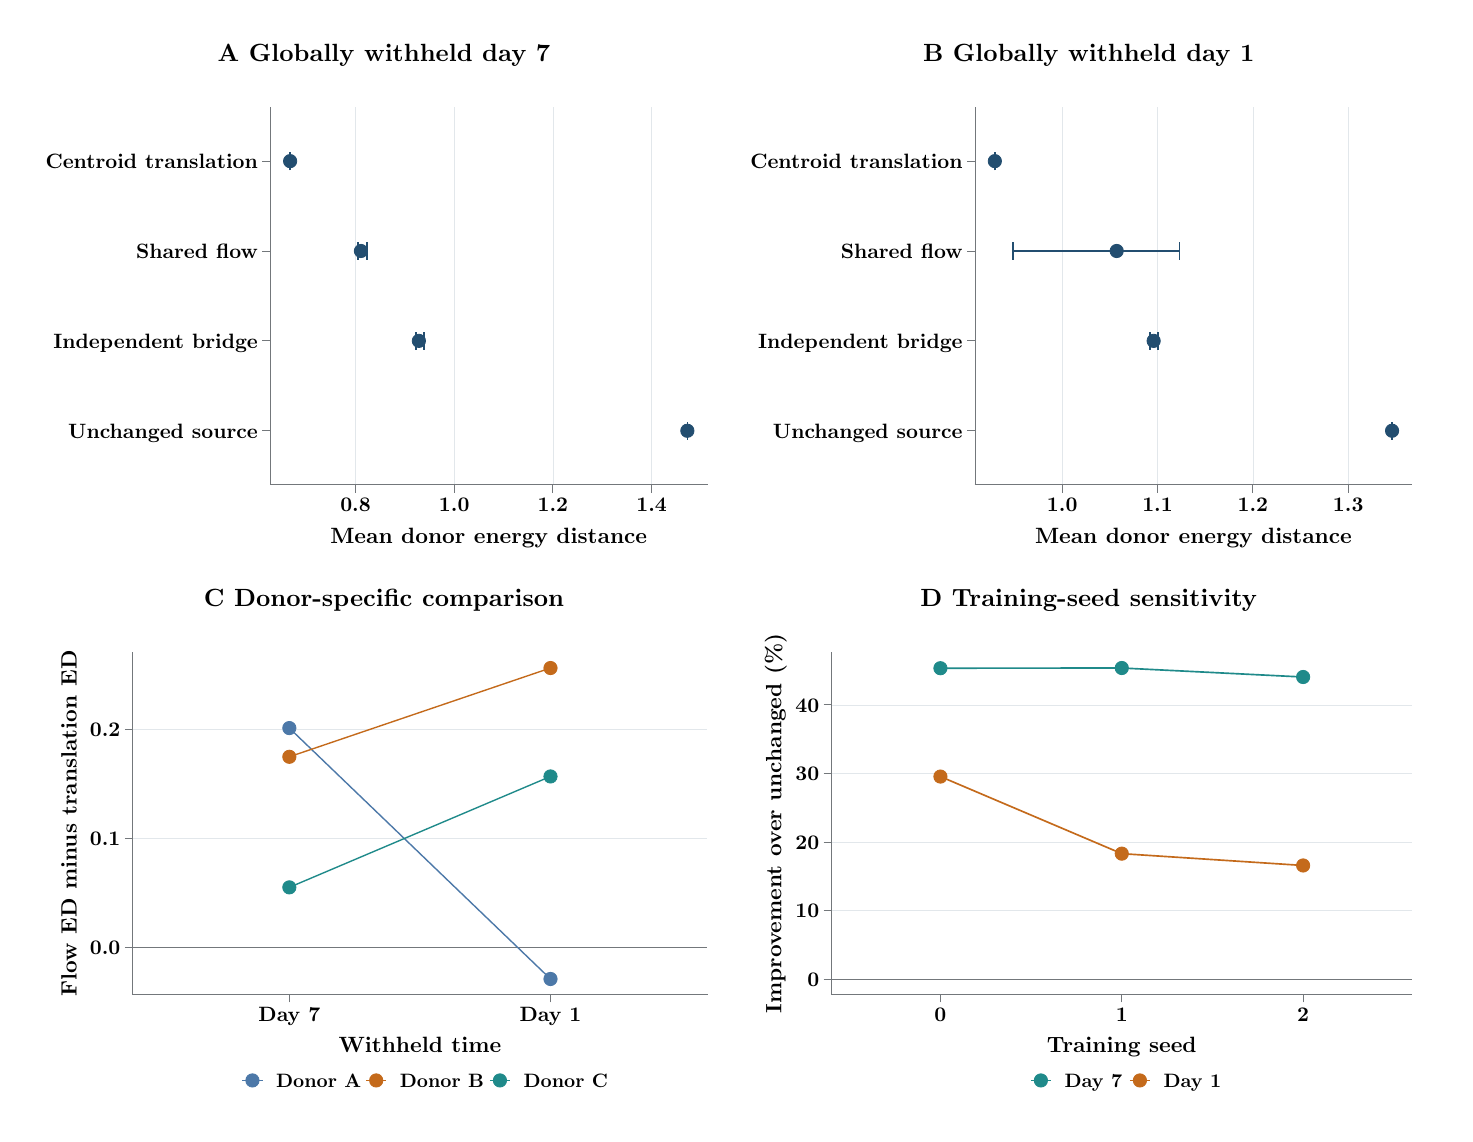
\begin{tikzpicture}[x=1pt,y=1pt]
\definecolor{fillColor}{RGB}{255,255,255}
\path[use as bounding box,fill=fillColor,fill opacity=0.00] (0,0) rectangle (512.15,392.65);
\begin{scope}
\path[clip] (  0.00,  0.00) rectangle (512.15,392.65);
\definecolor{drawColor}{RGB}{0,0,0}

\node[text=drawColor,anchor=base,inner sep=0pt, outer sep=0pt, scale=  0.90] at (128.75,380.52) {\bfseries A Globally withheld day 7};
\end{scope}
\begin{scope}
\path[clip] (  8.54,201.30) rectangle (248.96,369.03);
\definecolor{fillColor}{RGB}{255,255,255}

\path[fill=fillColor] (  8.54,201.30) rectangle (248.96,369.03);
\end{scope}
\begin{scope}
\path[clip] ( 87.65,227.50) rectangle (245.55,363.91);
\definecolor{fillColor}{RGB}{255,255,255}

\path[fill=fillColor] ( 87.65,227.50) rectangle (245.55,363.91);
\definecolor{drawColor}{RGB}{226,231,235}

\path[draw=drawColor,line width= 0.2pt,line join=round] (118.47,227.50) --
	(118.47,363.91);

\path[draw=drawColor,line width= 0.2pt,line join=round] (154.13,227.50) --
	(154.13,363.91);

\path[draw=drawColor,line width= 0.2pt,line join=round] (189.79,227.50) --
	(189.79,363.91);

\path[draw=drawColor,line width= 0.2pt,line join=round] (225.45,227.50) --
	(225.45,363.91);
\definecolor{drawColor}{RGB}{35,78,112}

\path[draw=drawColor,line width= 0.6pt,line join=round] (238.37,243.74) --
	(238.37,250.24);

\path[draw=drawColor,line width= 0.6pt,line join=round] (238.37,246.99) --
	(238.37,246.99);

\path[draw=drawColor,line width= 0.6pt,line join=round] (238.37,243.74) --
	(238.37,250.24);

\path[draw=drawColor,line width= 0.6pt,line join=round] ( 94.83,341.18) --
	( 94.83,347.67);

\path[draw=drawColor,line width= 0.6pt,line join=round] ( 94.83,344.42) --
	( 94.83,344.42);

\path[draw=drawColor,line width= 0.6pt,line join=round] ( 94.83,341.18) --
	( 94.83,347.67);

\path[draw=drawColor,line width= 0.6pt,line join=round] (143.18,276.22) --
	(143.18,282.72);

\path[draw=drawColor,line width= 0.6pt,line join=round] (143.18,279.47) --
	(140.30,279.47);

\path[draw=drawColor,line width= 0.6pt,line join=round] (140.30,276.22) --
	(140.30,282.72);

\path[draw=drawColor,line width= 0.6pt,line join=round] (122.69,308.70) --
	(122.69,315.19);

\path[draw=drawColor,line width= 0.6pt,line join=round] (122.69,311.95) --
	(119.25,311.95);

\path[draw=drawColor,line width= 0.6pt,line join=round] (119.25,308.70) --
	(119.25,315.19);
\definecolor{fillColor}{RGB}{35,78,112}

\path[draw=drawColor,line width= 0.3pt,line join=round,line cap=round,fill=fillColor] (238.37,246.99) circle (  2.40);

\path[draw=drawColor,line width= 0.3pt,line join=round,line cap=round,fill=fillColor] ( 94.83,344.42) circle (  2.40);

\path[draw=drawColor,line width= 0.3pt,line join=round,line cap=round,fill=fillColor] (141.36,279.47) circle (  2.40);

\path[draw=drawColor,line width= 0.3pt,line join=round,line cap=round,fill=fillColor] (120.42,311.95) circle (  2.40);
\end{scope}
\begin{scope}
\path[clip] (  0.00,  0.00) rectangle (512.15,392.65);
\definecolor{drawColor}{RGB}{115,119,123}

\path[draw=drawColor,line width= 0.3pt,line join=round,line cap=rect] ( 87.65,227.50) --
	( 87.65,363.91);
\end{scope}
\begin{scope}
\path[clip] (  0.00,  0.00) rectangle (512.15,392.65);
\definecolor{drawColor}{RGB}{0,0,0}

\node[text=drawColor,anchor=base east,inner sep=0pt, outer sep=0pt, scale=  0.75] at ( 83.20,244.31) {\bfseries Unchanged source};

\node[text=drawColor,anchor=base east,inner sep=0pt, outer sep=0pt, scale=  0.75] at ( 83.20,276.78) {\bfseries Independent bridge};

\node[text=drawColor,anchor=base east,inner sep=0pt, outer sep=0pt, scale=  0.75] at ( 83.20,309.26) {\bfseries Shared flow};

\node[text=drawColor,anchor=base east,inner sep=0pt, outer sep=0pt, scale=  0.75] at ( 83.20,341.74) {\bfseries Centroid translation};
\end{scope}
\begin{scope}
\path[clip] (  0.00,  0.00) rectangle (512.15,392.65);
\definecolor{drawColor}{RGB}{115,119,123}

\path[draw=drawColor,line width= 0.3pt,line join=round] ( 84.80,246.99) --
	( 87.65,246.99);

\path[draw=drawColor,line width= 0.3pt,line join=round] ( 84.80,279.47) --
	( 87.65,279.47);

\path[draw=drawColor,line width= 0.3pt,line join=round] ( 84.80,311.95) --
	( 87.65,311.95);

\path[draw=drawColor,line width= 0.3pt,line join=round] ( 84.80,344.42) --
	( 87.65,344.42);
\end{scope}
\begin{scope}
\path[clip] (  0.00,  0.00) rectangle (512.15,392.65);
\definecolor{drawColor}{RGB}{115,119,123}

\path[draw=drawColor,line width= 0.3pt,line join=round,line cap=rect] ( 87.65,227.50) --
	(245.55,227.50);
\end{scope}
\begin{scope}
\path[clip] (  0.00,  0.00) rectangle (512.15,392.65);
\definecolor{drawColor}{RGB}{115,119,123}

\path[draw=drawColor,line width= 0.3pt,line join=round] (118.47,224.66) --
	(118.47,227.50);

\path[draw=drawColor,line width= 0.3pt,line join=round] (154.13,224.66) --
	(154.13,227.50);

\path[draw=drawColor,line width= 0.3pt,line join=round] (189.79,224.66) --
	(189.79,227.50);

\path[draw=drawColor,line width= 0.3pt,line join=round] (225.45,224.66) --
	(225.45,227.50);
\end{scope}
\begin{scope}
\path[clip] (  0.00,  0.00) rectangle (512.15,392.65);
\definecolor{drawColor}{RGB}{0,0,0}

\node[text=drawColor,anchor=base,inner sep=0pt, outer sep=0pt, scale=  0.75] at (118.47,217.69) {\bfseries 0.8};

\node[text=drawColor,anchor=base,inner sep=0pt, outer sep=0pt, scale=  0.75] at (154.13,217.69) {\bfseries 1.0};

\node[text=drawColor,anchor=base,inner sep=0pt, outer sep=0pt, scale=  0.75] at (189.79,217.69) {\bfseries 1.2};

\node[text=drawColor,anchor=base,inner sep=0pt, outer sep=0pt, scale=  0.75] at (225.45,217.69) {\bfseries 1.4};
\end{scope}
\begin{scope}
\path[clip] (  0.00,  0.00) rectangle (512.15,392.65);
\definecolor{drawColor}{RGB}{0,0,0}

\node[text=drawColor,anchor=base,inner sep=0pt, outer sep=0pt, scale=  0.80] at (166.60,206.40) {\bfseries Mean donor energy distance};
\end{scope}
\begin{scope}
\path[clip] (  0.00,  0.00) rectangle (512.15,392.65);
\definecolor{drawColor}{RGB}{0,0,0}

\node[text=drawColor,anchor=base,inner sep=0pt, outer sep=0pt, scale=  0.90] at (383.40,380.52) {\bfseries B Globally withheld day 1};
\end{scope}
\begin{scope}
\path[clip] (263.19,201.30) rectangle (503.61,369.03);
\definecolor{fillColor}{RGB}{255,255,255}

\path[fill=fillColor] (263.19,201.30) rectangle (503.61,369.03);
\end{scope}
\begin{scope}
\path[clip] (342.30,227.50) rectangle (500.20,363.91);
\definecolor{fillColor}{RGB}{255,255,255}

\path[fill=fillColor] (342.30,227.50) rectangle (500.20,363.91);
\definecolor{drawColor}{RGB}{226,231,235}

\path[draw=drawColor,line width= 0.2pt,line join=round] (373.84,227.50) --
	(373.84,363.91);

\path[draw=drawColor,line width= 0.2pt,line join=round] (408.28,227.50) --
	(408.28,363.91);

\path[draw=drawColor,line width= 0.2pt,line join=round] (442.73,227.50) --
	(442.73,363.91);

\path[draw=drawColor,line width= 0.2pt,line join=round] (477.17,227.50) --
	(477.17,363.91);
\definecolor{drawColor}{RGB}{35,78,112}

\path[draw=drawColor,line width= 0.6pt,line join=round] (493.02,243.74) --
	(493.02,250.24);

\path[draw=drawColor,line width= 0.6pt,line join=round] (493.02,246.99) --
	(493.02,246.99);

\path[draw=drawColor,line width= 0.6pt,line join=round] (493.02,243.74) --
	(493.02,250.24);

\path[draw=drawColor,line width= 0.6pt,line join=round] (349.48,341.18) --
	(349.48,347.67);

\path[draw=drawColor,line width= 0.6pt,line join=round] (349.48,344.42) --
	(349.48,344.42);

\path[draw=drawColor,line width= 0.6pt,line join=round] (349.48,341.18) --
	(349.48,347.67);

\path[draw=drawColor,line width= 0.6pt,line join=round] (408.51,276.22) --
	(408.51,282.72);

\path[draw=drawColor,line width= 0.6pt,line join=round] (408.51,279.47) --
	(405.54,279.47);

\path[draw=drawColor,line width= 0.6pt,line join=round] (405.54,276.22) --
	(405.54,282.72);

\path[draw=drawColor,line width= 0.6pt,line join=round] (416.23,308.70) --
	(416.23,315.19);

\path[draw=drawColor,line width= 0.6pt,line join=round] (416.23,311.95) --
	(356.08,311.95);

\path[draw=drawColor,line width= 0.6pt,line join=round] (356.08,308.70) --
	(356.08,315.19);
\definecolor{fillColor}{RGB}{35,78,112}

\path[draw=drawColor,line width= 0.3pt,line join=round,line cap=round,fill=fillColor] (493.02,246.99) circle (  2.40);

\path[draw=drawColor,line width= 0.3pt,line join=round,line cap=round,fill=fillColor] (349.48,344.42) circle (  2.40);

\path[draw=drawColor,line width= 0.3pt,line join=round,line cap=round,fill=fillColor] (406.87,279.47) circle (  2.40);

\path[draw=drawColor,line width= 0.3pt,line join=round,line cap=round,fill=fillColor] (393.51,311.95) circle (  2.40);
\end{scope}
\begin{scope}
\path[clip] (  0.00,  0.00) rectangle (512.15,392.65);
\definecolor{drawColor}{RGB}{115,119,123}

\path[draw=drawColor,line width= 0.3pt,line join=round,line cap=rect] (342.30,227.50) --
	(342.30,363.91);
\end{scope}
\begin{scope}
\path[clip] (  0.00,  0.00) rectangle (512.15,392.65);
\definecolor{drawColor}{RGB}{0,0,0}

\node[text=drawColor,anchor=base east,inner sep=0pt, outer sep=0pt, scale=  0.75] at (337.86,244.31) {\bfseries Unchanged source};

\node[text=drawColor,anchor=base east,inner sep=0pt, outer sep=0pt, scale=  0.75] at (337.86,276.78) {\bfseries Independent bridge};

\node[text=drawColor,anchor=base east,inner sep=0pt, outer sep=0pt, scale=  0.75] at (337.86,309.26) {\bfseries Shared flow};

\node[text=drawColor,anchor=base east,inner sep=0pt, outer sep=0pt, scale=  0.75] at (337.86,341.74) {\bfseries Centroid translation};
\end{scope}
\begin{scope}
\path[clip] (  0.00,  0.00) rectangle (512.15,392.65);
\definecolor{drawColor}{RGB}{115,119,123}

\path[draw=drawColor,line width= 0.3pt,line join=round] (339.46,246.99) --
	(342.30,246.99);

\path[draw=drawColor,line width= 0.3pt,line join=round] (339.46,279.47) --
	(342.30,279.47);

\path[draw=drawColor,line width= 0.3pt,line join=round] (339.46,311.95) --
	(342.30,311.95);

\path[draw=drawColor,line width= 0.3pt,line join=round] (339.46,344.42) --
	(342.30,344.42);
\end{scope}
\begin{scope}
\path[clip] (  0.00,  0.00) rectangle (512.15,392.65);
\definecolor{drawColor}{RGB}{115,119,123}

\path[draw=drawColor,line width= 0.3pt,line join=round,line cap=rect] (342.30,227.50) --
	(500.20,227.50);
\end{scope}
\begin{scope}
\path[clip] (  0.00,  0.00) rectangle (512.15,392.65);
\definecolor{drawColor}{RGB}{115,119,123}

\path[draw=drawColor,line width= 0.3pt,line join=round] (373.84,224.66) --
	(373.84,227.50);

\path[draw=drawColor,line width= 0.3pt,line join=round] (408.28,224.66) --
	(408.28,227.50);

\path[draw=drawColor,line width= 0.3pt,line join=round] (442.73,224.66) --
	(442.73,227.50);

\path[draw=drawColor,line width= 0.3pt,line join=round] (477.17,224.66) --
	(477.17,227.50);
\end{scope}
\begin{scope}
\path[clip] (  0.00,  0.00) rectangle (512.15,392.65);
\definecolor{drawColor}{RGB}{0,0,0}

\node[text=drawColor,anchor=base,inner sep=0pt, outer sep=0pt, scale=  0.75] at (373.84,217.69) {\bfseries 1.0};

\node[text=drawColor,anchor=base,inner sep=0pt, outer sep=0pt, scale=  0.75] at (408.28,217.69) {\bfseries 1.1};

\node[text=drawColor,anchor=base,inner sep=0pt, outer sep=0pt, scale=  0.75] at (442.73,217.69) {\bfseries 1.2};

\node[text=drawColor,anchor=base,inner sep=0pt, outer sep=0pt, scale=  0.75] at (477.17,217.69) {\bfseries 1.3};
\end{scope}
\begin{scope}
\path[clip] (  0.00,  0.00) rectangle (512.15,392.65);
\definecolor{drawColor}{RGB}{0,0,0}

\node[text=drawColor,anchor=base,inner sep=0pt, outer sep=0pt, scale=  0.80] at (421.25,206.40) {\bfseries Mean donor energy distance};
\end{scope}
\begin{scope}
\path[clip] (  0.00,  0.00) rectangle (512.15,392.65);
\definecolor{drawColor}{RGB}{0,0,0}

\node[text=drawColor,anchor=base,inner sep=0pt, outer sep=0pt, scale=  0.90] at (128.75,183.48) {\bfseries C Donor-specific comparison};
\end{scope}
\begin{scope}
\path[clip] (  8.54,  4.27) rectangle (248.96,172.00);
\definecolor{fillColor}{RGB}{255,255,255}

\path[fill=fillColor] (  8.54,  4.27) rectangle (248.96,172.00);
\end{scope}
\begin{scope}
\path[clip] ( 37.93, 43.27) rectangle (245.55,166.88);
\definecolor{fillColor}{RGB}{255,255,255}

\path[fill=fillColor] ( 37.93, 43.27) rectangle (245.55,166.88);
\definecolor{drawColor}{RGB}{226,231,235}

\path[draw=drawColor,line width= 0.2pt,line join=round] ( 37.93, 60.44) --
	(245.55, 60.44);

\path[draw=drawColor,line width= 0.2pt,line join=round] ( 37.93, 99.78) --
	(245.55, 99.78);

\path[draw=drawColor,line width= 0.2pt,line join=round] ( 37.93,139.13) --
	(245.55,139.13);
\definecolor{drawColor}{RGB}{115,119,123}

\path[draw=drawColor,line width= 0.3pt,line join=round] ( 37.93, 60.44) -- (245.55, 60.44);
\definecolor{drawColor}{RGB}{76,120,168}

\path[draw=drawColor,line width= 0.5pt,line join=round] ( 94.55,139.56) --
	(188.92, 48.89);
\definecolor{drawColor}{RGB}{196,106,27}

\path[draw=drawColor,line width= 0.5pt,line join=round] ( 94.55,129.18) --
	(188.92,161.26);
\definecolor{drawColor}{RGB}{31,138,138}

\path[draw=drawColor,line width= 0.5pt,line join=round] ( 94.55, 82.00) --
	(188.92,122.08);
\definecolor{drawColor}{RGB}{76,120,168}
\definecolor{fillColor}{RGB}{76,120,168}

\path[draw=drawColor,line width= 0.3pt,line join=round,line cap=round,fill=fillColor] (188.92, 48.89) circle (  2.40);
\definecolor{drawColor}{RGB}{196,106,27}
\definecolor{fillColor}{RGB}{196,106,27}

\path[draw=drawColor,line width= 0.3pt,line join=round,line cap=round,fill=fillColor] (188.92,161.26) circle (  2.40);
\definecolor{drawColor}{RGB}{31,138,138}
\definecolor{fillColor}{RGB}{31,138,138}

\path[draw=drawColor,line width= 0.3pt,line join=round,line cap=round,fill=fillColor] (188.92,122.08) circle (  2.40);
\definecolor{drawColor}{RGB}{76,120,168}
\definecolor{fillColor}{RGB}{76,120,168}

\path[draw=drawColor,line width= 0.3pt,line join=round,line cap=round,fill=fillColor] ( 94.55,139.56) circle (  2.40);
\definecolor{drawColor}{RGB}{196,106,27}
\definecolor{fillColor}{RGB}{196,106,27}

\path[draw=drawColor,line width= 0.3pt,line join=round,line cap=round,fill=fillColor] ( 94.55,129.18) circle (  2.40);
\definecolor{drawColor}{RGB}{31,138,138}
\definecolor{fillColor}{RGB}{31,138,138}

\path[draw=drawColor,line width= 0.3pt,line join=round,line cap=round,fill=fillColor] ( 94.55, 82.00) circle (  2.40);
\end{scope}
\begin{scope}
\path[clip] (  0.00,  0.00) rectangle (512.15,392.65);
\definecolor{drawColor}{RGB}{115,119,123}

\path[draw=drawColor,line width= 0.3pt,line join=round,line cap=rect] ( 37.93, 43.27) --
	( 37.93,166.88);
\end{scope}
\begin{scope}
\path[clip] (  0.00,  0.00) rectangle (512.15,392.65);
\definecolor{drawColor}{RGB}{0,0,0}

\node[text=drawColor,anchor=base east,inner sep=0pt, outer sep=0pt, scale=  0.75] at ( 33.49, 57.75) {\bfseries 0.0};

\node[text=drawColor,anchor=base east,inner sep=0pt, outer sep=0pt, scale=  0.75] at ( 33.49, 97.10) {\bfseries 0.1};

\node[text=drawColor,anchor=base east,inner sep=0pt, outer sep=0pt, scale=  0.75] at ( 33.49,136.45) {\bfseries 0.2};
\end{scope}
\begin{scope}
\path[clip] (  0.00,  0.00) rectangle (512.15,392.65);
\definecolor{drawColor}{RGB}{115,119,123}

\path[draw=drawColor,line width= 0.3pt,line join=round] ( 35.09, 60.44) --
	( 37.93, 60.44);

\path[draw=drawColor,line width= 0.3pt,line join=round] ( 35.09, 99.78) --
	( 37.93, 99.78);

\path[draw=drawColor,line width= 0.3pt,line join=round] ( 35.09,139.13) --
	( 37.93,139.13);
\end{scope}
\begin{scope}
\path[clip] (  0.00,  0.00) rectangle (512.15,392.65);
\definecolor{drawColor}{RGB}{115,119,123}

\path[draw=drawColor,line width= 0.3pt,line join=round,line cap=rect] ( 37.93, 43.27) --
	(245.55, 43.27);
\end{scope}
\begin{scope}
\path[clip] (  0.00,  0.00) rectangle (512.15,392.65);
\definecolor{drawColor}{RGB}{115,119,123}

\path[draw=drawColor,line width= 0.3pt,line join=round] ( 94.55, 40.43) --
	( 94.55, 43.27);

\path[draw=drawColor,line width= 0.3pt,line join=round] (188.92, 40.43) --
	(188.92, 43.27);
\end{scope}
\begin{scope}
\path[clip] (  0.00,  0.00) rectangle (512.15,392.65);
\definecolor{drawColor}{RGB}{0,0,0}

\node[text=drawColor,anchor=base,inner sep=0pt, outer sep=0pt, scale=  0.75] at ( 94.55, 33.46) {\bfseries Day 7};

\node[text=drawColor,anchor=base,inner sep=0pt, outer sep=0pt, scale=  0.75] at (188.92, 33.46) {\bfseries Day 1};
\end{scope}
\begin{scope}
\path[clip] (  0.00,  0.00) rectangle (512.15,392.65);
\definecolor{drawColor}{RGB}{0,0,0}

\node[text=drawColor,anchor=base,inner sep=0pt, outer sep=0pt, scale=  0.80] at (141.74, 22.17) {\bfseries Withheld time};
\end{scope}
\begin{scope}
\path[clip] (  0.00,  0.00) rectangle (512.15,392.65);
\definecolor{drawColor}{RGB}{0,0,0}

\node[text=drawColor,rotate= 90.00,anchor=base,inner sep=0pt, outer sep=0pt, scale=  0.80] at ( 17.68,105.07) {\bfseries Flow ED minus translation ED};
\end{scope}
\begin{scope}
\path[clip] (  0.00,  0.00) rectangle (512.15,392.65);
\definecolor{fillColor}{RGB}{255,255,255}

\path[fill=fillColor] ( 76.67,  7.68) rectangle (206.81, 16.79);
\end{scope}
\begin{scope}
\path[clip] (  0.00,  0.00) rectangle (512.15,392.65);
\definecolor{fillColor}{RGB}{255,255,255}

\path[fill=fillColor] ( 76.67,  7.68) rectangle ( 85.78, 16.79);
\definecolor{drawColor}{RGB}{76,120,168}

\path[draw=drawColor,line width= 0.5pt,line join=round] ( 77.58, 12.23) -- ( 84.87, 12.23);
\definecolor{fillColor}{RGB}{76,120,168}

\path[draw=drawColor,line width= 0.3pt,line join=round,line cap=round,fill=fillColor] ( 81.22, 12.23) circle (  2.40);
\end{scope}
\begin{scope}
\path[clip] (  0.00,  0.00) rectangle (512.15,392.65);
\definecolor{fillColor}{RGB}{255,255,255}

\path[fill=fillColor] (121.38,  7.68) rectangle (130.49, 16.79);
\definecolor{drawColor}{RGB}{196,106,27}

\path[draw=drawColor,line width= 0.5pt,line join=round] (122.29, 12.23) -- (129.58, 12.23);
\definecolor{fillColor}{RGB}{196,106,27}

\path[draw=drawColor,line width= 0.3pt,line join=round,line cap=round,fill=fillColor] (125.94, 12.23) circle (  2.40);
\end{scope}
\begin{scope}
\path[clip] (  0.00,  0.00) rectangle (512.15,392.65);
\definecolor{fillColor}{RGB}{255,255,255}

\path[fill=fillColor] (166.09,  7.68) rectangle (175.20, 16.79);
\definecolor{drawColor}{RGB}{31,138,138}

\path[draw=drawColor,line width= 0.5pt,line join=round] (167.01, 12.23) -- (174.29, 12.23);
\definecolor{fillColor}{RGB}{31,138,138}

\path[draw=drawColor,line width= 0.3pt,line join=round,line cap=round,fill=fillColor] (170.65, 12.23) circle (  2.40);
\end{scope}
\begin{scope}
\path[clip] (  0.00,  0.00) rectangle (512.15,392.65);
\definecolor{drawColor}{RGB}{0,0,0}

\node[text=drawColor,anchor=base west,inner sep=0pt, outer sep=0pt, scale=  0.70] at ( 89.78,  9.73) {\bfseries Donor A};
\end{scope}
\begin{scope}
\path[clip] (  0.00,  0.00) rectangle (512.15,392.65);
\definecolor{drawColor}{RGB}{0,0,0}

\node[text=drawColor,anchor=base west,inner sep=0pt, outer sep=0pt, scale=  0.70] at (134.49,  9.73) {\bfseries Donor B};
\end{scope}
\begin{scope}
\path[clip] (  0.00,  0.00) rectangle (512.15,392.65);
\definecolor{drawColor}{RGB}{0,0,0}

\node[text=drawColor,anchor=base west,inner sep=0pt, outer sep=0pt, scale=  0.70] at (179.20,  9.73) {\bfseries Donor C};
\end{scope}
\begin{scope}
\path[clip] (  0.00,  0.00) rectangle (512.15,392.65);
\definecolor{drawColor}{RGB}{0,0,0}

\node[text=drawColor,anchor=base,inner sep=0pt, outer sep=0pt, scale=  0.90] at (383.40,183.48) {\bfseries D Training-seed sensitivity};
\end{scope}
\begin{scope}
\path[clip] (263.19,  4.27) rectangle (503.61,172.00);
\definecolor{fillColor}{RGB}{255,255,255}

\path[fill=fillColor] (263.19,  4.27) rectangle (503.61,172.00);
\end{scope}
\begin{scope}
\path[clip] (290.50, 43.27) rectangle (500.20,166.88);
\definecolor{fillColor}{RGB}{255,255,255}

\path[fill=fillColor] (290.50, 43.27) rectangle (500.20,166.88);
\definecolor{drawColor}{RGB}{226,231,235}

\path[draw=drawColor,line width= 0.2pt,line join=round] (290.50, 48.89) --
	(500.20, 48.89);

\path[draw=drawColor,line width= 0.2pt,line join=round] (290.50, 73.66) --
	(500.20, 73.66);

\path[draw=drawColor,line width= 0.2pt,line join=round] (290.50, 98.42) --
	(500.20, 98.42);

\path[draw=drawColor,line width= 0.2pt,line join=round] (290.50,123.19) --
	(500.20,123.19);

\path[draw=drawColor,line width= 0.2pt,line join=round] (290.50,147.95) --
	(500.20,147.95);
\definecolor{drawColor}{RGB}{115,119,123}

\path[draw=drawColor,line width= 0.3pt,line join=round] (290.50, 48.89) -- (500.20, 48.89);
\definecolor{drawColor}{RGB}{31,138,138}

\path[draw=drawColor,line width= 0.6pt,line join=round] (329.82,161.19) --
	(395.35,161.26) --
	(460.88,158.01);
\definecolor{drawColor}{RGB}{196,106,27}

\path[draw=drawColor,line width= 0.6pt,line join=round] (329.82,122.04) --
	(395.35, 94.18) --
	(460.88, 89.91);
\definecolor{drawColor}{RGB}{31,138,138}
\definecolor{fillColor}{RGB}{31,138,138}

\path[draw=drawColor,line width= 0.3pt,line join=round,line cap=round,fill=fillColor] (329.82,161.19) circle (  2.40);

\path[draw=drawColor,line width= 0.3pt,line join=round,line cap=round,fill=fillColor] (395.35,161.26) circle (  2.40);

\path[draw=drawColor,line width= 0.3pt,line join=round,line cap=round,fill=fillColor] (460.88,158.01) circle (  2.40);
\definecolor{drawColor}{RGB}{196,106,27}
\definecolor{fillColor}{RGB}{196,106,27}

\path[draw=drawColor,line width= 0.3pt,line join=round,line cap=round,fill=fillColor] (329.82,122.04) circle (  2.40);

\path[draw=drawColor,line width= 0.3pt,line join=round,line cap=round,fill=fillColor] (395.35, 94.18) circle (  2.40);

\path[draw=drawColor,line width= 0.3pt,line join=round,line cap=round,fill=fillColor] (460.88, 89.91) circle (  2.40);
\end{scope}
\begin{scope}
\path[clip] (  0.00,  0.00) rectangle (512.15,392.65);
\definecolor{drawColor}{RGB}{115,119,123}

\path[draw=drawColor,line width= 0.3pt,line join=round,line cap=rect] (290.50, 43.27) --
	(290.50,166.88);
\end{scope}
\begin{scope}
\path[clip] (  0.00,  0.00) rectangle (512.15,392.65);
\definecolor{drawColor}{RGB}{0,0,0}

\node[text=drawColor,anchor=base east,inner sep=0pt, outer sep=0pt, scale=  0.75] at (286.05, 46.21) {\bfseries 0};

\node[text=drawColor,anchor=base east,inner sep=0pt, outer sep=0pt, scale=  0.75] at (286.05, 70.97) {\bfseries 10};

\node[text=drawColor,anchor=base east,inner sep=0pt, outer sep=0pt, scale=  0.75] at (286.05, 95.74) {\bfseries 20};

\node[text=drawColor,anchor=base east,inner sep=0pt, outer sep=0pt, scale=  0.75] at (286.05,120.50) {\bfseries 30};

\node[text=drawColor,anchor=base east,inner sep=0pt, outer sep=0pt, scale=  0.75] at (286.05,145.27) {\bfseries 40};
\end{scope}
\begin{scope}
\path[clip] (  0.00,  0.00) rectangle (512.15,392.65);
\definecolor{drawColor}{RGB}{115,119,123}

\path[draw=drawColor,line width= 0.3pt,line join=round] (287.65, 48.89) --
	(290.50, 48.89);

\path[draw=drawColor,line width= 0.3pt,line join=round] (287.65, 73.66) --
	(290.50, 73.66);

\path[draw=drawColor,line width= 0.3pt,line join=round] (287.65, 98.42) --
	(290.50, 98.42);

\path[draw=drawColor,line width= 0.3pt,line join=round] (287.65,123.19) --
	(290.50,123.19);

\path[draw=drawColor,line width= 0.3pt,line join=round] (287.65,147.95) --
	(290.50,147.95);
\end{scope}
\begin{scope}
\path[clip] (  0.00,  0.00) rectangle (512.15,392.65);
\definecolor{drawColor}{RGB}{115,119,123}

\path[draw=drawColor,line width= 0.3pt,line join=round,line cap=rect] (290.50, 43.27) --
	(500.20, 43.27);
\end{scope}
\begin{scope}
\path[clip] (  0.00,  0.00) rectangle (512.15,392.65);
\definecolor{drawColor}{RGB}{115,119,123}

\path[draw=drawColor,line width= 0.3pt,line join=round] (329.82, 40.43) --
	(329.82, 43.27);

\path[draw=drawColor,line width= 0.3pt,line join=round] (395.35, 40.43) --
	(395.35, 43.27);

\path[draw=drawColor,line width= 0.3pt,line join=round] (460.88, 40.43) --
	(460.88, 43.27);
\end{scope}
\begin{scope}
\path[clip] (  0.00,  0.00) rectangle (512.15,392.65);
\definecolor{drawColor}{RGB}{0,0,0}

\node[text=drawColor,anchor=base,inner sep=0pt, outer sep=0pt, scale=  0.75] at (329.82, 33.46) {\bfseries 0};

\node[text=drawColor,anchor=base,inner sep=0pt, outer sep=0pt, scale=  0.75] at (395.35, 33.46) {\bfseries 1};

\node[text=drawColor,anchor=base,inner sep=0pt, outer sep=0pt, scale=  0.75] at (460.88, 33.46) {\bfseries 2};
\end{scope}
\begin{scope}
\path[clip] (  0.00,  0.00) rectangle (512.15,392.65);
\definecolor{drawColor}{RGB}{0,0,0}

\node[text=drawColor,anchor=base,inner sep=0pt, outer sep=0pt, scale=  0.80] at (395.35, 22.17) {\bfseries Training seed};
\end{scope}
\begin{scope}
\path[clip] (  0.00,  0.00) rectangle (512.15,392.65);
\definecolor{drawColor}{RGB}{0,0,0}

\node[text=drawColor,rotate= 90.00,anchor=base,inner sep=0pt, outer sep=0pt, scale=  0.80] at (272.33,105.07) {\bfseries Improvement over unchanged ({\%})};
\end{scope}
\begin{scope}
\path[clip] (  0.00,  0.00) rectangle (512.15,392.65);
\definecolor{fillColor}{RGB}{255,255,255}

\path[fill=fillColor] (361.57,  7.68) rectangle (429.13, 16.79);
\end{scope}
\begin{scope}
\path[clip] (  0.00,  0.00) rectangle (512.15,392.65);
\definecolor{fillColor}{RGB}{255,255,255}

\path[fill=fillColor] (361.57,  7.68) rectangle (370.67, 16.79);
\definecolor{drawColor}{RGB}{31,138,138}

\path[draw=drawColor,line width= 0.6pt,line join=round] (362.48, 12.23) -- (369.76, 12.23);
\definecolor{fillColor}{RGB}{31,138,138}

\path[draw=drawColor,line width= 0.3pt,line join=round,line cap=round,fill=fillColor] (366.12, 12.23) circle (  2.40);
\end{scope}
\begin{scope}
\path[clip] (  0.00,  0.00) rectangle (512.15,392.65);
\definecolor{fillColor}{RGB}{255,255,255}

\path[fill=fillColor] (397.35,  7.68) rectangle (406.45, 16.79);
\definecolor{drawColor}{RGB}{196,106,27}

\path[draw=drawColor,line width= 0.6pt,line join=round] (398.26, 12.23) -- (405.54, 12.23);
\definecolor{fillColor}{RGB}{196,106,27}

\path[draw=drawColor,line width= 0.3pt,line join=round,line cap=round,fill=fillColor] (401.90, 12.23) circle (  2.40);
\end{scope}
\begin{scope}
\path[clip] (  0.00,  0.00) rectangle (512.15,392.65);
\definecolor{drawColor}{RGB}{0,0,0}

\node[text=drawColor,anchor=base west,inner sep=0pt, outer sep=0pt, scale=  0.70] at (374.67,  9.73) {\bfseries Day 7};
\end{scope}
\begin{scope}
\path[clip] (  0.00,  0.00) rectangle (512.15,392.65);
\definecolor{drawColor}{RGB}{0,0,0}

\node[text=drawColor,anchor=base west,inner sep=0pt, outer sep=0pt, scale=  0.70] at (410.45,  9.73) {\bfseries Day 1};
\end{scope}
\end{tikzpicture}

\end{document}
